\section{P3: CIFAR-10 Transfer with a Compact CNN}
\label{sec:p3-cifar10}

P3 asks whether the final Event-FedAvg operating point transfers beyond the
Fashion-MNIST evidence used to develop the method. The protocol was frozen
before held-out inspection. It uses the official CIFAR-10 training and test
sets, ten equal clients, and a deterministic strong-label-skew partition: client
$i$ receives 2750 examples of class $i$ and 250 examples of every other class.
The conventional compact CNN has two strided convolutional layers, one hidden
fully connected layer, and 20,570 trainable parameters. This is not an SNN; the
neuromorphic inspiration remains confined to the communication operator.

All methods use 120 synchronous full-participation rounds, five local SGD steps
per round, minibatches of 32, learning rate 0.05, and $5\times10^{-4}$ L2
regularization. Configuration selection uses partition seed 3400 only. The
untouched held-out partitions are 3500, 3600, and 3700, with method-matched
initialization and minibatch streams. Communication includes packet headers,
coordinate addresses, initial model synchronization, uplink and downlink, and
the cheaper of exact sparse replay and dense checkpointing. The headline cost
is conservative bidirectional unicast traffic.

% Generated by paper/ijcnn2027/build_evidence.py; do not edit by hand.
\begin{table*}[t]
\centering
\caption{CIFAR-10 results over three held-out data realizations. Values are mean $\pm$ sample standard deviation; total is conservative bidirectional unicast traffic. Quality-selected and nearest-traffic rows are separated.}
\label{tab:cifar10-results}
\small
\begin{tabular}{llrrrr}
\toprule
Selection & Method & Test CE & Accuracy [\%] & Worst class [\%] & Total [Mbit] \\
\midrule
Quality & Event-FedAvg & 1.4411$\pm$0.0260 & 48.06$\pm$1.12 & 24.6$\pm$4.6 & 201.5$\pm$4.3 \\
Quality & Strom & 1.4529$\pm$0.0096 & 47.68$\pm$0.49 & 18.9$\pm$3.8 & 930.9$\pm$2.0 \\
Quality & EF-TopK & 1.6069$\pm$0.0078 & 42.19$\pm$0.37 & 26.7$\pm$0.8 & 645.2$\pm$0.0 \\
Quality & Sign-EF & 1.6395$\pm$0.0090 & 41.59$\pm$0.33 & 24.6$\pm$3.2 & 279.4$\pm$0.0 \\
Quality & Dense FedAvg & 1.5482$\pm$0.0285 & 44.13$\pm$1.12 & 23.3$\pm$5.6 & 1586.6$\pm$0.0 \\
\midrule
Nearest traffic & Event-FedAvg & 1.4411$\pm$0.0260 & 48.06$\pm$1.12 & 24.6$\pm$4.6 & 201.5$\pm$4.3 \\
Nearest traffic & Strom & 1.8040$\pm$0.1284 & 35.50$\pm$4.00 & 10.3$\pm$3.8 & 221.8$\pm$14.8 \\
Nearest traffic & EF-TopK & 1.6461$\pm$0.0084 & 40.95$\pm$0.14 & 23.6$\pm$0.5 & 135.3$\pm$0.0 \\
\bottomrule
\end{tabular}
\end{table*}


\begin{figure}[t]
  \centering
  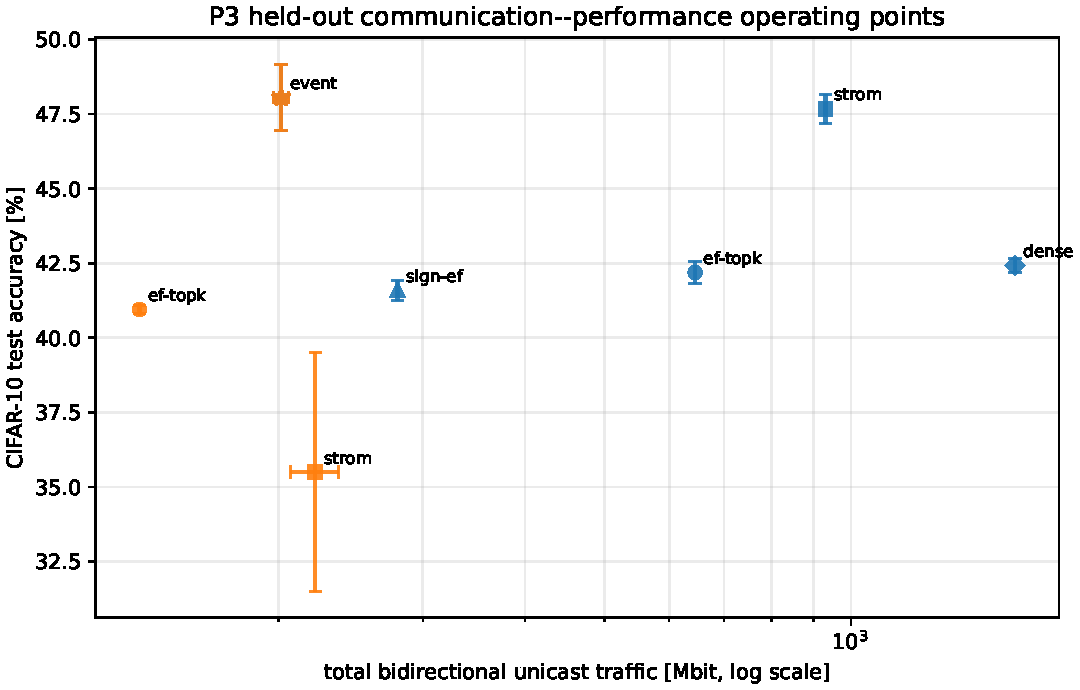
\includegraphics[width=0.96\linewidth]{figures/p3_cifar10_frontier.pdf}
  \caption{Held-out CIFAR-10 communication--performance operating points.
  Blue points are development quality-selected configurations and orange
  points are the nearest development traffic controls; Event-FedAvg is common
  to both comparisons. Error bars show one sample standard deviation over
  three untouched partitions. Event-FedAvg is nondominated and uses far less
  total traffic than every quality-selected baseline.}
  \label{fig:p3-cifar10-frontier}
\end{figure}

Event-FedAvg obtains $48.06\pm1.12\%$ mean test accuracy and
$1.4411\pm0.0260$ test cross-entropy at $201.5\pm4.3$ Mbit. Dense FedAvg obtains
$42.42\pm0.24\%$ at 1586.6 Mbit. Thus the event method uses 12.7\% of dense
traffic, a 7.9-fold reduction, while its mean accuracy is 5.63 percentage
points higher. It also uses less traffic and has higher mean accuracy than
each quality-selected compressed baseline. In particular, quality-selected
Strom reaches $47.68\pm0.49\%$ but requires $930.9\pm2.0$ Mbit.

The nearest-neighbor comparison is intentionally read as an operating-point
test rather than exact traffic equality. The nearest Strom point is 10.1\%
more expensive than Event-FedAvg and 12.56 percentage points less accurate.
The nearest EF-TopK point is 32.9\% cheaper and 7.10 percentage points less
accurate, so neither strictly dominates the other. This control therefore
supports a favorable Event-FedAvg trade-off without erasing the low-traffic
EF-TopK alternative.

The predeclared P3 gate is a \textbf{pass}: Event-FedAvg remains on the
communication--performance frontier on a second dataset and architecture.
The boundary matters. Only three held-out seeds were evaluated, so no
statistical-significance claim is made. Mean worst-class accuracy is slightly
lower than dense FedAvg and quality-selected EF-TopK and has appreciable
between-partition variation. The campaign also remains synchronous and
full-participation, and its bit accounting is not a hardware-energy or measured
network-latency result.
